\chapter{How to Have an Impactful Role in the Company}

This lecture begins with a practical question and then answers it by a controlled rewind. We are asked what the day-to-day work was and what part of it proved most impactful, but the speaker does not begin with a finished job description. He begins with a path. If we want to see why the role mattered, we must first see how its boundary widened: from a narrow commercial assignment, to the full customer-facing surface of the company, and then into its operating core. There is little literal mathematics on the page here, but there is a precise organizational mechanics, and it is worth writing that mechanics carefully.

\section{The Question and the Rewind}

The opening question asks for two things at once: the daily work itself, and the most impactful part of it. The answer does not come immediately. The speaker says, in effect, that we must drop back and look at the journey. That is not a digression. It is the method of the lecture.

We therefore read the transcript as a sequence of state changes. The object that changes is the set of functions for which the speaker has direct responsibility. Once we see that set expand, the answer to the original question begins to emerge on its own.

\section{A Small Initial Role}

At the beginning, the role is narrow enough to write explicitly. Let \(R\) denote the bundle of functions directly under the speaker's responsibility at a given moment. The initial bundle is
\begin{equation}
R_0 = \{\text{commercial sales},\ \text{account management}\}.
\end{equation}

\begin{definition}
Throughout this chapter, \(R\) denotes a responsibility bundle: the set of business functions for which the speaker is directly accountable at a given stage of the narrative.
\end{definition}

This notation is useful because the lecture is not really about titles. It is about the movement of a boundary. The initial condition is simple: a commercial role with account-management responsibility. Only after we have this starting point can we measure what the later enlargements mean.

\section{The First Expansion: Everything That Touched the Customer}

After about a year, the head of federal and state leaves, and the CEO tells him to take over those areas as well. The lecture then proceeds in two passes. First there is the immediate reassignment, and then there is the speaker's fuller recap of what the resulting bundle had become.

\paragraph{Worked update rule.}
If we keep close to the spoken sequence, the first update may be written as
\begin{align}
t_{\mathrm{expand}} &\approx 1\ \text{year},\\
R_0 &\longrightarrow R_0 \cup \{\text{state},\ \text{federal}\}.
\end{align}
But the transcript does not stop with that minimal change. The speaker continues by enumerating the broader bundle he in fact carried:
\begin{equation}
R_1 =
\{\text{commercial},\ \text{state},\ \text{federal},\ \text{sales},\ \text{account management},\ \text{marketing},\ \text{government relations}\}.
\end{equation}

The list is intentionally left a little rough, because it is spoken, not extracted from a formal org chart. In particular, ``commercial'' and ``sales'' may overlap. That untidiness is part of the point: the lecturer is conveying the felt growth of the role before he abstracts it.

\begin{definition}
Let \(R_{\mathrm{cust}}\) denote the bundle of functions that, in the speaker's own phrase, ``touched a customer'' at HMS.
\end{definition}

\begin{equation}
R_1 \approx R_{\mathrm{cust}}.
\end{equation}

\begin{remark}
The symbol \(\approx\) is deliberate. The transcript gives us a spoken list and then a summarizing phrase, not a formally audited equality of departments.
\end{remark}

Now the narrative reaches its first plateau. The speaker can summarize his position by saying that he ran everything at HMS that touched a customer. This is the first place where the opening question begins to receive a genuine answer.

\subsection{Question \& Answer}

\paragraph{Question.}
At this stage, what makes the role impactful: the rank attached to it, or the breadth of the bundle \(R\)?

\paragraph{Answer.}
The lecture points to breadth. Once \(R\) has grown to something like \(R_{\mathrm{cust}}\), the role is no longer a narrow sales assignment. It has become the company's customer-facing boundary. Impact appears here as scope: the speaker is now governing the surface on which the firm meets the market.

\section{Scale and Stability}

The transcript immediately strengthens that answer by adding two anchors. The first is a scale marker. The second is a time marker. At the time, HMS was running at roughly \$400 million, and this customer-facing bundle lasted not for a few weeks but for years.

\begin{align}
\mathrm{RunRate}_{\mathrm{HMS}} &\approx \$400\,\mathrm{M},\\
t_{\mathrm{cust}} &\approx 4\ \text{years}.
\end{align}

These quantities keep the story from sounding anecdotal. A customer-touching boundary at this scale is economically consequential, and a four-year tenure in that configuration means we are not looking at a temporary overlap of duties. We are looking at a stable operating regime.

This is also where the lecture becomes more deliberate in its internal logic. First the speaker enlarges the bundle. Then he shows that the enlarged bundle is big enough to matter and stable enough to count. Only after that does he move to the next pivot.

\section{The Second Expansion: From Interface to Operations}

After those four years, a new problem appears: one division is facing a major challenge. Here the rhythm changes. The first expansion came from vacancy and reassignment. The second comes from trouble in the business and from the speaker's own request to take charge of it.

To make this move possible, someone else is brought in to run the client-facing side. The speaker then says that he ultimately took over the COB business, the payment integrity business, and the IT shop. We write
\begin{equation}
R_{\mathrm{ops}} = \{\text{COB},\ \text{payment integrity},\ \text{IT}\}.
\end{equation}

The whole narrative may now be compressed into a single transition law:
\begin{equation}
R_0
\xrightarrow{\text{CEO adds state/federal}}
R_{\mathrm{cust}}
\xrightarrow{\text{division challenge}+\text{handoff}}
R_{\mathrm{ops}}.
\end{equation}

\begin{figure}
\begin{center}
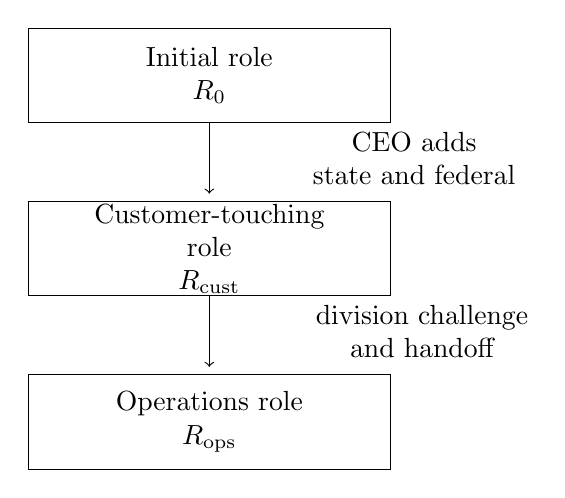
\begin{tikzpicture}[x=1cm,y=1cm]
\draw (0,4.4) rectangle (4.6,5.6);
\node[align=center] at (2.3,5.0) {Initial role\\\(R_0\)};

\draw[->] (2.3,4.4) -- (2.3,3.5);
\node[align=center] at (4.9,3.95) {CEO adds\\state and federal};

\draw (0,2.2) rectangle (4.6,3.4);
\node[align=center] at (2.3,2.8) {Customer-touching\\role\\\(R_{\mathrm{cust}}\)};

\draw[->] (2.3,2.2) -- (2.3,1.3);
\node[align=center] at (5.0,1.75) {division challenge\\and handoff};

\draw (0,0.0) rectangle (4.6,1.2);
\node[align=center] at (2.3,0.6) {Operations role\\\(R_{\mathrm{ops}}\)};
\end{tikzpicture}
\end{center}
\end{figure}

The diagram is a cautious reconstruction from the transcript alone, but it captures the lecture's geometry. The path is not merely upward. It moves inward: from the customer interface to the machinery by which the company actually performs.

\subsection{Question \& Answer}

\paragraph{Question.}
If the speaker already ran everything that touched a customer, why does this later move sound even more consequential?

\paragraph{Answer.}
Because the second transition changes not only the size of the bundle but the kind of leverage it carries. Customer-facing control governs the interface. Operational control governs the internal process from which outcomes are produced. The lecture's implied claim is that impact deepens when responsibility passes from contact to execution.

\section{The Meaning of the Final Pivot}

The closing sentence of the excerpt is garbled and repeats itself, but its direction is still intelligible. The speaker is trying to distinguish a fully external-facing role from running the operations of the company. We should therefore keep the contrast, but not overstate it. The transcript does not license a polished doctrine; it gives us a clear direction with slightly damaged wording.

What matters is the asymmetry between the two transitions. In the first, the speaker becomes responsible for more of what the customer sees. In the second, he becomes responsible for more of what produces the company's result. This is why the lecture feels like an answer to the original question rather than a list of promotions. Impact is being located at the point where scope, scale, and operating consequence meet.

\section{Summary}

The lecture starts from a practical question and answers it by reconstructing the widening boundary of a role. We begin with
\begin{equation}
R_0 = \{\text{commercial sales},\ \text{account management}\},
\end{equation}
we enlarge that bundle until it is approximately the full customer-facing surface \(R_{\mathrm{cust}}\), we attach scale and duration to show that this scope is real, and we finally pass to an operating bundle
\begin{equation}
R_{\mathrm{ops}} = \{\text{COB},\ \text{payment integrity},\ \text{IT}\}.
\end{equation}
The chapter's central lesson is therefore not a slogan about leadership. It is a structural claim: impact grows as the boundary of responsibility grows, and it grows again when that boundary moves from the market-facing edge of the firm into the core of its operations.